\documentclass{SCreport}
\usepackage[utf8]{inputenc}
\usepackage[T1]{fontenc}
\usepackage{caption}
\usepackage{float}
\captionsetup{font=small}
\setcounter{tocdepth}{2}
\newcommand\h[1]{\hspace{#1}}
\newcommand\I[1]{\rule{0pt}{#1}}
\reporttype{SC21}
\reportauthor{A.~Magnusson\footnote{\spc}, N.~Davies\footnote{TeTakina Ltd},
  G.~Pilling$^1$, P.~Hamer$^1$}
\reporttitle{Scoping the Next Generation of Tuna Stock Assessment
  Software:\\Progress Report and Outline of Options (Project 123)}
\reportnumber{\tpnum/SA-WP-01}
\reportdate{14 July 2025}
\setlength\tolerance{2000}
\hyphenation{decisions future supported assessments acknowledged marlin software
  assessment replacement consideration development traditional collaboration
  benefits exercises embarking}
\begin{document}

\wcpfctitlepage

\tableofcontents
\newpage

\section{Executive summary}

The 3-year Project 123 aims to evaluate features and capabilities that will be
important in future tuna assessments, explore fitting models to tuna data using
existing software platforms, guide decisions on the type of new software
development required, and establish collaboration with tuna Regional Fisheries
Management Organizations (RFMOs) and research labs to achieve these goals.

At SC20, ISG-09 reviewed the scoping of next-generation tuna stock assessment
software and supported prioritizing practical tasks, including transitioning
swordfish and striped marlin assessments to Stock Synthesis and testing
simplified models for yellowfin tuna. Members acknowledged the need to focus on
immediate assessment priorities while keeping longer-term software development
under consideration, depending on available resources and capacity. (SC20
Summary Report, Attachment E).

SC21 will review the progress of Project 123, which explores the transition to
next-generation stock assessment software for tuna fisheries. The project report
i) evaluates the benefits, limitations, uncertainties, and resource implications
associated with each software platform under consideration; ii) evaluates the
feasibility of analyzing tagging data independently from the main stock
assessment models, a potential strategy to reduce model complexity while
maintaining scientific robustness; and iii) identifies key analytical features
and technical capabilities that future stock assessment platforms should
incorporate, such as support for spatial structure, tagging integration, and
flexibility for multi-species and multi-fleet assessments, to ensure that WCPFC
assessments remain scientifically credible, transparent, and adaptable to
evolving fishery and management needs.

SC21 will provide feedback on the progress of the project as needed.

\vspace{4ex}

We invite SC21 to:

\begin{itemize}
  \item note that over the next 5+ years, MULTIFAN-CL will begin to be phased
  out as a software platform for WCPFC tuna and billfish stock assessments;
  \item note that in 2025, the two billfish stock assessments, swordfish and
  striped marlin, transitioned from MULTIFAN-CL to Stock Synthesis; and
  \item review and comment on two suggested software development work streams,
  described in this report and provide feedback that will guide the preparation
  of project proposals to be presented to SC22;
\end{itemize}

\newpage

\section{Introduction}

  % \item note that in 2024, a project workshop was conducted in Matapouri, New
  % Zealand, focusing on possible outcomes, options, and preparing for upcoming
  % activities;
  % \item note that in 2025, a technical evaluation of the RTMB programming
  % environment was carried out with worked examples;
  % \item note that in 2025, a technical workshop was conducted in Copenhagen,
  % Denmark, focusing on the development of a fine-scale spatio-temporal model for
  % external analysis of tagging data, producing abundance indices to be
  % incorporated into a tuna stock assessment;
  % \item note that in 2025, SPC reached out to the FIMS software project to
  % discuss the possibility of developing tuna-specific code modules to link with
  % core FIMS modules to construct models that meet the needs of tuna assessments;
  % \item note that in 2025, SPC reached out to the Gadget software project to
  % discuss the possibility of developing Gadget models to fit SPC tuna data, to
  % evaluate the usefulness of explicit age-length structure and other features of
  % Gadget relevant for tuna assessments;
  % \item SPC has reached out to the RFMOs
  % \item SPC has made a single-region yellowfin tuna dataset available online,
  % intented for comparing different assessment software platforms, and fitted a
  % MULTIFAN-CL model to this dataset

\subsection{The need to migrate to new software}

Following the retirement of the lead developer of MULTIFAN-CL (MFCL), Dave
Fournier, future advances to the MFCL software are not expected to be as
mathematically innovative as they were in the past. While this does not render
MFCL obsolete in the medium-term, it flags the need to plan and identify whether
alternative existing software exists, or new software must be developed in the
longer-term, to continue to support the specificities and future requirements of
WCPFC tuna stock assessments.

While MFCL (Fournier et al. 1998) continues to be improved to service the WCPFC
tuna assessment needs over at least the next 5+ years, it is important to start
on a phased approach to its replacement. An initial scoping phase is required to
assess what features and capabilities will be important in future assessment
software for tunas. This scoping phase will benefit from input from stock
assessment scientists across global tuna RFMOs. Once this scoping phase is
conducted, consideration of available software packages in relation to the
desired features and capabilities can be conducted. This may identify suitable
existing software that has potential to provide the desired features and/or has
potential to be developed further. Alternatively, it may indicate whether
embarking on development of a new software package is recommended.

There has also been discussion around the need to explore, through
modeling/simulation exercises, the benefits of applying alternative assessment
structures (i.e., length-age structured versus the traditional length-based
age-structured approach of MFCL and Stock Synthesis) before embarking on major
software developments or changing methodology. Similar can be said about
exploring benefits of state-space models and their use of random variables.
Simulation exercises to explore the benefits or drawbacks of alternative model
structures or approaches will also require collaboration across tuna RFMOs and
practitioners experienced in using the alternative approaches and/or software.

An important outcome of this work would be to ultimately have a software package
that has the desired functionality for tuna assessments, not only for WCPFC but
also for other tuna RFMOs, thus creating a user community and ongoing
development support capacity, so as to avoid the current situation we are facing
with MFCL. Wider collaboration in this venture is essential to achieving this
and is expected to be encouraged through this project.

\subsection{Project outline}
\label{sec:project-outline}

This scoping project is scheduled from 1 Feb 2024 to 31 Dec 2026. It will:

\begin{itemize}
  \item[-] evaluate features and capabilities that will be important in future
  tuna assessments\\[-4.5ex]
  \item[-] explore fitting models to tuna data using existing software
  platforms\\[-4.5ex]
  \item[-] guide decisions on what kind of new software development will be
  required\\[-4.5ex]
  \item[-] establish collaboration with tRFMOs and research labs to achieve
  these goals
\end{itemize}

Additional projects can be launched in parallel to power up the model
exploration and software development.

The project is divided into stages, as follows:

Year 2024

\begin{enumerate}
  \item Review and identify important features for tuna assessments.\\[-4.5ex]
  \item Identify existing software platforms that have these features or can be
  extended.\\[-4.5ex]
  \item Reach out to and initiate collaboration with model developers.\\[-4.5ex]
  \item Conduct two workshops in 2024, one online and one in person.\\
\end{enumerate}

Years 2025 and 2026 (subject to SC advice and funding approvals by WCPFC)

\begin{enumerate}\setcounter{enumi}{4}
  \item Explore and compare existing platforms, fitting to SPC tuna
  data.\\[-4.5ex]
  \item Determine which platforms can be considered viable candidates.\\[-4.5ex]
  \item If a viable candidate platform has been identified, plan
  transition.\\[-4.5ex]
  \item If no viable candidate platform is identified, launch a software
  development project\\
  to extend a platform or create a new one.
\end{enumerate}

\newpage

\subsection{Existing software}

The CAPAM 2019 Workshop on Next Generation Assessment Models (Punt et al. 2020)
provided an overview and discussion of existing software, as well as
recommendations for further software development.

For the purposes of tuna assessments, the most relevant existing software (other
than MFCL) includes:

\begin{itemize}
  \item \textbf{Stock Synthesis} is used in tuna assessments by the IATTC, IOTC,
  and ICCAT. Migrating SPC assessments to Stock Synthesis would lose some of the
  features provided by MFCL and this would be transitioning to another platform
  that is expected to be phased out in the not-too-distant future. On the other
  hand, increasing the use of Stock Synthesis at SPC would facilitate
  collaboration between the tRFMOs, including development of future models. It
  would also shorten the training time for new SPC stock assessors and make
  their skills and experience more transferable to subsequent workplaces. Stock
  Synthesis assessments would allow closer comparisons of assessments conducted
  across RFMOs and also SPC and the ISC. Stock Synthesis has a large user
  community that is relevant for peer reviews and discussing technical
  decisions. It also comes with an exceptionally complete suite of tools useful
  for diagnostics, as well as automated plots and tables for assessment reports.
  A possible avenue of collaborative development is to explore the possibility
  of enhancing the tag module, see \autoref{sec:ongoing-upcoming-development}.
  \item \textbf{sbt} is used in the assessment of southern bluefin tuna by
  CCSBT. This package, implemented in TMB, stands out as the primary stock
  assessment software that is built around close-kin mark-recapture (CKMR) which
  is a new and important data type in upcoming SPC tuna assessments. The
  \textsf{sbt} R package is designed for a single-region assessment and would
  require some additional development to be used for a multiregion assessment. A
  possible avenue of collaborative development is to explore the possibility of
  adding multiregion functionality to the software.
  \item \textbf{Gadget3} is the latest version of Gadget stock assessment
  platform, implemented in TMB. It is an age-length structured platform and
  porting the software to TMB has resulted in a significant performance gain in
  terms of computational time. Gadget has a wide range of features relevant for
  tuna assessments and a possible avenue of collaborative development is to test
  the use of Gadget for a tuna assessment.
  \item \textbf{Casal2} is the latest version of the Casal stock assessment
  platform, rewritten with an improved design and user interface. Casal has a
  wide range of features relevant for tuna assessments and a possible avenue of
  collaborative development is to test the use of Casal for a tuna assessment.
  \newpage
  \item \textbf{Stock Synthesis + CKMR} is an experimental add-on to Stock
  Synthesis (A.E. Punt, pers. comm), adding CKMR as a data type in Stock
  Synthesis. This was successful as a proof of concept but it is unlikely to be
  added to the core software.
  \item \textbf{ALSCL} is a recent model (Zhang and Cadigan 2022) that has two
  important features: state-space formulation and age-length structure. It is
  implemented in TMB, but the software currently fits only to survey data and
  does not include commercial catches or fleets. A possible avenue of
  collaborative development is to explore the ability of this model to analyze a
  simplified tuna dataset. This would provide insights into the dynamics of
  fitting state-space age-length models in general and also be a first step
  before considering extensions to the model further, see ALSCL + Fleets below.
\end{itemize}

\subsection{Ongoing and upcoming software development}
\label{sec:ongoing-upcoming-development}

Some ongoing software development projects are of particular interest in the
context of the next WCPFC tuna assessment models:

\begin{itemize}
  \item \textbf{Stock Synthesis + Enhanced Tags} is a proposed software
  development of an enhanced tag module for Stock Synthesis. The current
  implementation of fitting to tagging data is somewhat limited, e.g., requiring
  the user to enter the age at release, which is not available in tuna
  assessments. The idea is to borrow some of the functionality and features from
  the tag module in MFCL, which has a long record of using tagging data as a
  primary data type in tuna assessments. A possible avenue of collaborative
  development is to explore the possibility of contributing an enhanced tag
  module to be incorporated into the core Stock Synthesis software.
  \item \textbf{WHAM + Length} is a recent software development (Correa et al.
  2023) extending the state-space stock assessment software WHAM (Stock and
  Miller 2021) to fit to length data. A possible avenue of collaborative
  development is to experiment with fitting the WHAM + Length model to an SPC
  tuna assessment dataset.
  \item \textbf{ALSCL + Fleets} is a potential software development extending
  the ALSCL model to address the primary shortcomings of the current ALSCL model
  as candidate software for tuna stock assessments. A possible avenue of
  collaborative development is to explore the possibility of adding commercial
  catches and fleets as software features.
  \item \textbf{SAM + Length} is an early exploration of extending the
  state-space stock assessment software SAM (Nielsen and Berg 2014) to fit to
  length data. A possible avenue of collaborative development is to continue
  this exploration.
  \newpage
  \item \textbf{FIMS} is a NOAA project that coordinates the development of a
  next-generation framework of stock assessment models based on TMB. So far,
  model development within FIMS has focused on models fitting to age data. It is
  not clear at this point whether the FIMS project will lead to stock assessment
  software that can be used in tuna assessments, but given the considerable
  resources and collaborative nature of the project, SPC will communicate and
  interact with the FIMS project to share development progress and ideas.
\end{itemize}

Model features that are important for future tuna assessment models are reviewed
by Punt et al. (2020), Hoyle et al. (2020), and Magnusson and Davies (2024).

Advice on the management and structure of a software development project is
provided by Hoyle et al. (2020), covering topics such as design, programming
paradigms, maintenance tools, and user interface.

\section{Possible tasks for SPC to prioritize}
\label{sec:possible-tasks}

This section discusses core areas for ongoing work, and proposed activities to
be considered in each area. We reiterate that progression from MFCL to an
alternative software is not a `side project' that can be subsumed within the
current SSP resourcing. For this reason we suggest that a small informal working
group could be convened by the SC to discuss and prioritise activities that
would require additional resources, and develop TORs for priority activities.

\subsection{Migrate assessments to existing software}

\begin{enumerate}
  \item Move the swordfish assessment to Stock Synthesis. The Southwest Pacific
  swordfish assessment model is relatively simple compared to other SPC
  assessments and would be a good candidate to be the first to migrate from
  MFCL. The 2025 swordfish assessment could be developed in a stepwise
  progression: previous MFCL diagnostic $\Rightarrow$ catch-conditioned MFCL
  $\Rightarrow$ Stock Synthesis.
  \item Move the striped marlin assessment to Stock Synthesis. The striped
  marlin assessment model is also relatively simple and would be a good
  candidate to migrate from MFCL. The next striped marlin assessment, currently
  scheduled in 2029, could be developed in a stepwise progression: previous
  catch-conditioned MFCL diagnostic $\Rightarrow$ Stock Synthesis.
\end{enumerate}

\subsection{Model exploration using existing software}

\begin{enumerate}\setcounter{enumi}{2}
  \item Conduct model exploration to fit Casal/Gadget/Stock Synthesis to
  albacore tuna. The South Pacific albacore assessment model is simpler than the
  other tuna species and therefore a candidate to be the~first tuna stock
  assessment to consider for migration from MFCL. Also, for the next South
  Pacific albacore assesmsent there may be CKMR information available to
  incorporate in the assessment.
  \item Conduct model exploration to fit Casal/Gadget/Stock Synthesis to the
  original five-region yellowfin tuna dataset. The yellowfin assessment is a
  good candidate to test the capabilities of these software platforms for tuna
  assessments involving multiple regions, tags, and a large number of fisheries.
  The yellowfin tuna assessment is similar to bigeye tuna but runs slightly
  faster, thanks to the simpler \mbox{five-region} structure that was adopted in
  the 2023 assessment.
  \item Conduct model exploration to fit models using a variety of existing
  software to a simplified single-region yellowfin tuna dataset. Models of
  interest include ALSCL, Casal, Gadget, MFCL, sbt, Stock Synthesis, and
  WHAM+Length.
\end{enumerate}

\subsection{Software development}

\subsubsection{Extend existing software}

The benefits and rationale of the following software extensions are described in
\autoref{sec:ongoing-upcoming-development}. The prioritization and duration of
these tasks may depend on the initial findings of these and other tasks,
available resources, and the availability of external scientists involved.

\begin{enumerate}\setcounter{enumi}{5}
  \item ALSCL+Fleets. Scientists involved could include Fan Zhang (Shanghai
  Ocean University) and Nick Davies (SPC consultant).
  \item Stock Synthesis+Enhanced Tags. Scientists involved could include
  Nicholas Ducharme-Barth (NOAA), Matthew Vincent (NOAA), and Arni Magnusson
  (SPC).
  \item WHAM+Length. Scientists involved could include Giancarlo Correa (AZTI)
  and Arni Magnusson (SPC).
  \item SAM+Length. Scientists involved could include Anders Nielsen (DTU),
  Colin Millar (ICES), and Arni Magnusson (SPC).
\end{enumerate}

\subsubsection{Design and develop new software for tuna assessments}

\begin{enumerate}\setcounter{enumi}{9}
  \item Initial explorations using RTMB, starting with simple model development
  and gradually adding complexity and tests. Scientists involved could include
  Nick Davies (SPC consultant) and Arni Magnusson (SPC).
\end{enumerate}

\section{Timeline}

\subsection{Pre-assessment workshop 2024}

An initial outline and discussion of project 123 was presented (Magnusson and
Davies 2024a) at the pre-assessment workshop at SPC headquarters on 28 March
2024. It provided a summary of existing software platforms and ongoing software
development projects, a roadmap of the project, and highlighted the need for
increased resources needed to conduct model exploration and software
development.

\subsection{International expert meeting 2024}

Two online meetings were held on 13 May and 18 June 2024, inviting stock
assessment and software development experts from around the world. Around 40
participants represented the tuna RFMOs (CCSBT, IATTC, ICCAT, IOTC, WCPFC),
stock assessment software projects (ALSCL, CASAL, FIMS, Gadget, MFCL, SAM, sbt,
Stock Synthesis, WHAM), and relevant programming environments (ADMB, RTMB, TMB).
See participant list in \autoref{sec:meeting-participants}.

\subsubsection{Objectives}

The meeting objectives were:

\begin{enumerate}
  \item Communicate SPC scoping project and upcoming explorations, decisions,
  and development.
  \item Discuss succession plans for MULTIFAN-CL as well as Stock Synthesis.
  \item Seek advice from the scientific community.
  \item Seek collaboration with tuna RFMOs and various research labs.
\end{enumerate}

\subsubsection{Format}

The two sessions had the same format and agenda, but one was centered on
European time zones and the other on North American time zones. The meeting
agenda covered the following discussion topics:

\begin{itemize}
  \item Platforms currently used in tuna stock assessments\\[-4ex]
  \item Common challenges for all tuna RFMOs, longevity of Stock Synthesis and
  MULTIFAN-CL, succession plans\\[-4ex]
  \item SPC challenges and project plan\\[-4ex]
  \item Features of current and future platforms\\[-4ex]
  \item Discussion on platform features most relevant for tuna\\[-4ex]
  \item State-space models and latest developments\\[-4ex]
  \item What do you think is the best way forward for SPC?\\[-4ex]
  \item Summary of discussions, next steps, collaboration
\end{itemize}

\subsubsection{Outcomes}

The following recommendations emerged from the discussions at the international
expert meeting:

\begin{enumerate}
  \item \textbf{Tuna assessment software.} There was a consensus among the
  experts that the goal should be to design and develop a model specific for
  tuna assessments, rather than a general model for global usage and all
  species. The advice was to start with a lean design and get a simple model up
  and running before adding all the features required for an assessment. In
  general, the cost of adding features is much greater than the implementation
  cost, as each layer complexity makes long-term maintenance and future
  modifications of the software more difficult and costly.
  \item \textbf{RTMB as a lean software development paradigm.} RTMB (Kristensen
  2024) is a new alternative interface for developing TMB (Kristensen et al.
  2017) models. RTMB provides a leaner development paradigm than TMB. The
  recommendation from the TMB/RTMB development team, articulated at the expert
  meeting, was to develop the next tuna stock assessment model in RTMB rather
  than TMB. Another recommendation from the TMB/RTMB development team, given the
  streamlined nature of RTMB model implementation is for SPC to consider writing
  specific models for each species, rather than a general platform for all
  species and tRFMOs. A specific RTMB model requires a very small codebase that
  is easy to maintain and modify. Parts of code can still be reused between
  species, either as code blocks or functions.
  \item \textbf{State-space formulation.} State-space models are a statistically
  and computationally efficient way to allow time-varying processes in stock
  assessment models, such as time-varying selectivity. Other statistical
  approaches exist, but the successful track record of using state-space models
  in production assessments, e.g., across a variety of Atlantic groundfish
  stocks, indicates that state-space formulation can be recommended for new
  model development.
  \item \textbf{Age-length structure.} Gadget models explicitly track the
  population by age and length, accounting for the fact that fast-growing
  individuals are caught by the fishery and the slow-growing individuals in the
  cohort remain in the population. Casal and Stock Synthesis have optional model
  features with a similar aim. This leads to an improved level of realism, and
  simulations using a very basic model ALSCL (Zhang and Cadigan 2022) indicate
  improved estimation accuracy. It is worth noting that the ALSCL simulation
  study involved a single-area model with survey data and no commercial catch
  data or fleets, which is quite far from the model complexity of tuna
  assessments. An important drawback is that tracking the population structure
  in terms of age and length, instead of age only, comes at a considerable
  computational cost. The SPC tuna assessment models that are currently run in
  MFCL are already very computationally heavy, with models requiring to run
  overnight before results are available. The recommendation is to explore the
  feature of incorporating full age-length structure in the next tuna assessment
  models, considering estimation performance and the difference in the resulting
  management advice, as well as computational time, required software
  development, and maintenance cost.
  \item \textbf{Simple models.} SPC challenges were outlined and discussed at
  the meeting, focusing on the upcoming paradigm change in how stock assessments
  are conducted at SPC. The MFCL Team (Dave Fournier, John Hampton, Nick Davies)
  will be retiring in the 2020s. Other stock assessment staff tend to have a
  relatively quick turnover rate, often consisting of young scientists with
  relatively few years of stock assessment experience before they start their
  job at SPC. It takes many years to become an expert in MFCL, with John Hampton
  typically making the main modeling decisions and guiding new staff, with the
  help of Nick Davies. Generally, it is preferable to have some long-term staff
  in the stock assessment team, but it is precautionary and prudent to prepare
  for an era where there might be no long-term staff, only short-term. In
  software design terms, this would favor not only a simple and intuitive user
  interface but also simpler assessment models than have been used in the past.
  \item \textbf{Collaboration between tuna
    RFMOs.}\label{item:collaboration-rfmos} For undertaking tuna assessments
  that fit to length composition data from multiple fisheries, SPC uses MFCL,
  while other tuna RFMOs use primarily Stock Synthesis. Both software platforms
  are currently in a sunset phase, heading towards end of life in the coming
  years. Development of new features in MFCL and Stock Synthesis is slowing
  down, with resources being allocated to succession plans. For SPC, it would be
  preferable to avoid developing and maintaining major software products that
  are not used outside of SPC. The statistical challenges of analyzing tuna data
  are comparable between the tuna RFMOs, noting some differences like degree of
  tagging data, so it makes sense to coordinate and collaborate in succession
  plans and new software development.
\end{enumerate}

The discussion at the international expert meeting covered several other topics,
but the above recommendations are particularly relevant for initial explorations
and development. The presentations from the international expert meeting are
available online (\autoref{sec:deliverables}). In addition to the discussion and
recommendations, an important outcome of the international expert meeting was to
establish collaboration with various research labs related to the development of
new tuna assessment models. See next section.

\subsection{Workshop activities in 2024--2026}

The first steps in the scoping project 123 have involved a review of software
needs and existing software, an evaluation of options, establishing
collaborative ties with research labs, and reaching out to scientists from the
other tRFMOs for coordination and consultation. We expect that presentation of
the outcomes so far at SC21 will facilitate discussion and the feedback from SC
will guide which of the tasks listed in \autoref{sec:possible-tasks} will be
prioritized. Discussions at SC should help guide TORs for each year's successive
work.

Hands-on technical workshops will be conducted in 2024--2026 to strengthen
collaboration ties and make stepwise progress on tasks that have been selected
as priorities. If prioritized, the work on migrating billfish assessments (Tasks
1--2 in the list of tasks) will be conducted by SPC scientists independent of
project 123 workshops. Progress with model exploration using alternative
software (Tasks 3--5) and software development (Tasks 6--9), if prioritized,
will depend on the resources and number of staff and consultants engaged in
those tasks. Another factor is the availability and commitment of external
scientists and other tRFMOs.

\newpage

Project 123 includes a budget that can be used to invite selected external
scientists to attend technical workshops to collaborate with SPC scientists on
selected tasks. A workshop might be organized for a week, either at SPC
headquarters or at another convenient venue, and collaborative work conducted
before, during, and after a workshop.

The first hands-on technical workshop had been planned at SPC headquarters
around October--November 2024, inviting two scientists. However, the unrest in
New Caledonia in 2024 will prevent such a workshop being conducted at that time.

Instead, the first hands-on technical workshop will take place in New Zealand on
23--30 August 2024, with Nick Davies (SPC consultant) and Arni Magnusson (SPC)
meeting directly after the SC~meeting in Manila. The main objectives are to test
the functionality and capabilities of RTMB on simple models and to conduct
exploratory runs of the ALSCL model. The 2024 workshop will evaluate RTMB as a
programming environment and paradigm for further software development, exploring
technical aspects such as whether it would be practical to organize the majority
of source code behind an assessment model as scripts, a package, or more than
one package. This would determine how code is maintained and shared between
assessments of different species.

The 2024 workshop corresponds to Task 10 listed in \autoref{sec:possible-tasks}.
Focus topics for workshops in 2025 and 2026 will be selected based on which
tasks will be prioritized by the WCPFC Scientific Committee and SPC.

\subsection{Launching the main project}

The current annual budget of project 123 is sufficient for scoping the needs,
identifying current software platforms, reaching out to the scientific community
for consultation, and to conduct occasional workshops to strengthen
collaboration ties and initial explorations. This corresponds to the first line
in \autoref{fig:diagram} and objectives 1--4 in the project outline
(\autoref{sec:project-outline}).

The goal of the \emph{main project}, which could either overlap or succeed the
scoping project, is to test/develop tuna stock assessment software and
transition all SPC assessments from MFCL to other platforms. To make significant
progress on the steps required to complete the main project (see full diagram in
\autoref{fig:diagram}), thus achieving objectives 5--8 in the project outline
(\autoref{sec:project-outline}), a~substantially larger commitment of resources
will be required, see next section.

\begin{figure}[H]
  \centering
  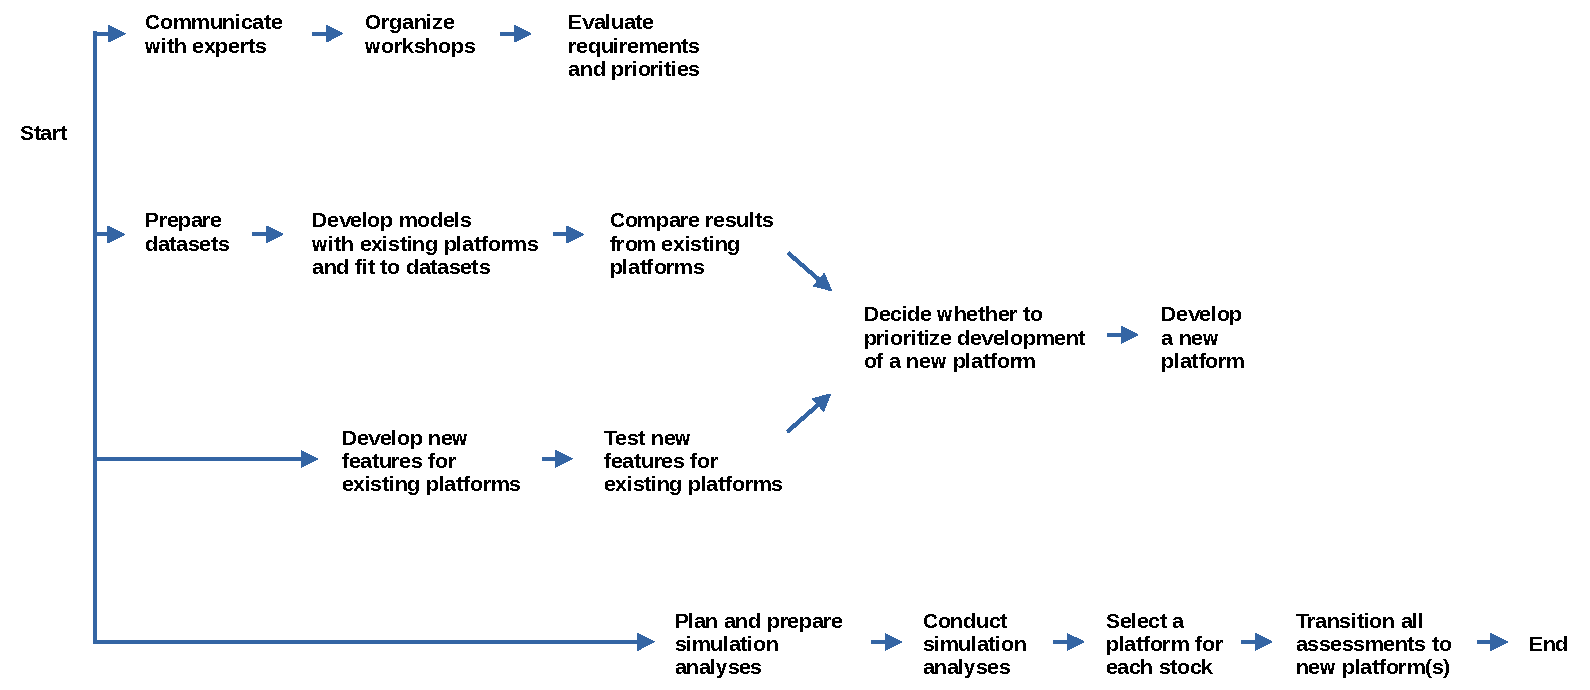
\includegraphics[width=\textwidth]{tasks_no_margin}
  \caption{Overview of steps related to the next generation of tuna stock
    assessment software. Project~123 will focus on the first line of scoping
    tasks (communicate, organize, evaluate) and prepare the ground for
    subsequent lines of tasks (the main project), which will require additional
    funding and resources.}\label{fig:diagram}
\end{figure}

\section{Required resources}

\subsection{Collaboration with other tRFMOs}

There are significant potential benefits for the tuna RFMOs to coordinate
together and collaborate on succession plans and new software development
(expert meeting recommendation \ref{item:collaboration-rfmos}). Coordination and
collaboration has already begun between tuna stock assessment scientists, with
one-on-one consultation meetings before and after the 2024 international expert
meeting.

The next step is for the tRFMOs to discuss financial and staff commitments to
formalize and strengthen collaboration related to succession plans and new
software development. Projects to accomplish the tasks laid out in
\autoref{fig:diagram} will require considerable resources. To achieve the
desired rate of progress and scientific quality of the end result, each tRFMO
could hire/assign one full-time person to the project for five years, or until
assessments have been transitioned to the new software.

\subsection{SPC staff positions, consultants}

The research and development required to test, design and develop stock
assessment software and successfully transition all SPC assessments from MFCL to
other platforms is difficult to estimate precisely, in terms of budget and time.
It is clear, however, that it will likely to take several years for a newly
formed team consisting of SPC staff scientists and/or consultants, along with
collaborators from other tRFMOs and research labs. To succeed, this team should
be primarily assigned to this project and not committed to the traditional stock
assessment related tasks and workflows. There is interaction between the roles
of a \emph{project coordinator}, \emph{fisheries scientist}, and \emph{software
  developer}, but it would be helpful for the project to define the role of each
staff scientist and consultant as clearly as possible, to accurately measure the
resources committed to the main project.

The resources committed to the main project will determine the scientific
quality of the end result and the number of years it takes to transition all SPC
assessments from MFCL to other platforms. Now that the first author of MFCL,
David Fournier, has retired, it would be highly beneficial for the project to
move relatively fast, before the remaining MFCL team (John Hampton and Nick
Davies) retire and will no longer be available for consultation and involvement
regarding software design, testing and technical decisions.

Compared to the other tuna RFMOs, there is greater urgency for WCPFC to move
this project forward. Independent of decisions and commitments of the other tuna
RFMOs, the main project would probably require one staff to be dedicated to this
work initially and depending on the direction taken (i.e., use pre-existing
software vs. develop new software) an additional staff or consultant with
software development skills. It is likely that transitioning MFCL assessments to
other software is at least a 5 year proposition, but there are some options to
begin this immediately with the simpler billfish assessments, and potentially
South Pacific albacore that need to prepare for the inclusion of CKMR data.

\section{Acknowledgements}

We thank WCPFC and ISSF for funding this scoping project. We are also grateful
for the valuable input of the scientists and software developers who joined the
online meetings of the 2024 international expert meeting.

\section{References}

\sloppy\setlength\hyphenpenalty{1000}

\begin{description}\setlength\itemsep{0ex}
  \item Correa, G.M., C.C. Monnahan, J.Y. Sullivan, J.T. Thorson, and A.E. Punt.
  2023. Modelling time-varying growth in state-space stock assessments. ICES J.
  Mar. Sci.80:2036--2049.
  \item Fournier, D.A., J. Hampton, and J.R. Sibert. 1998. MULTIFAN-CL: A
  length-based, age-structured model for fisheries stock assessment, with
  application to South Pacific albacore, \textit{Thunnus alalunga}. Can. J.
  Fish. Aquat. Sci. 55:2105--2116.
  \item Hoyle, S.D., M.N. Maunder, and Z.T. A'mar. 2020. Frameworks for the next
  generation of general stock assessment models: 2019 CAPAM workshop report. New
  Zealand Fish. Assess. Rep. 2020/39. 80 pp.
  \item Kristensen, K. 2024. RTMB: R bindings for TMB. R package version 1.5.\\
  \href{https://cran.r-project.org/package=RTMB}{https://cran.r-project.org/package=RTMB}.
  \item Kristensen, K. A. Nielsen, C.W. Berg, H. Skaug, and B.M. Bell. 2016.
  TMB: Automatic differentiation and Laplace approximation. J. Stat. Softw.
  70(5):1--21.
  \item Magnusson, A. and N. Davies. 2024a. Scoping the next stock assessment
  platform, P123: Background and discussion. Presented at the SPC pre-assessment
  workshop, 28 March 2024. 13 pp.
  \href{https://github.com/PacificCommunity/ofp-sam-transition-plan/blob/main/presentations/2024_03_28_paw_scoping/2024_03_28_paw_scoping.pdf}
  {Available online}.
  \item Magnusson, A. and N. Davies. 2024b. Scoping the next stock assessment
  platform, stage I:\linebreak Reaching out to tuna RFMOs and the scientific
  community. Presented at the SPC international expert meeting, 13 May and 18
  June 2024. 31 pp.
  \href{https://github.com/PacificCommunity/ofp-sam-transition-plan/blob/main/presentations/2024_05_13_experts_scoping/2024_05_13_experts_scoping.pdf}
  {Available online}.
  \item Nielsen, A. and C.W. Berg. 2014. Estimation of time-varying selectivity
  in stock assessments using state-space models. Fish. Res. 158:96--101.
  \item Punt, A.E., A. Dunn, B.Þ. Elvarsson, J. Hampton, S.D. Hoyle, M.N.
  Maunder, R.D. Methot, and A. Nielsen. 2020. Essential features of the
  next-generation integrated fisheries stock assessment package: A perspective.
  Fish. Res. 229:105617.
  \item Stock, B.C. and T.J. Miller. 2021. The Woods Hole Assessment Model
  (WHAM): A general state-space assessment framework that incorporates time- and
  age-varying processes via random effects and links to environmental
  covariates. Fish. Res. 240:105967.
  \item Zhang, F. and N.G. Cadigan. 2022. An age-and length-structured
  statistical catch-at-length model for hard-to-age fisheries stocks. Fish and
  Fish. 23:1121--1135.
\end{description}

\newpage

\appendix

\section{Appendices}

\subsection{Participants in the international expert meeting 2024}
\label{sec:meeting-participants}

\vspace{2ex}

\begin{tabular}{lll}
  \hline
  Name                    & Affiliation          & Country\\
  \hline
  Agurtzane Urtizberea    & AZTI                 & Spain\I{2.8ex}\\
  Ai Kimoto               & ICCAT                & Spain\\
  Alistair Dunn           & Ocean Environmental  & NZ\\
  Anders Nielsen          & DTU Aqua             & Denmark\\
  Andre Punt              & Univ Washington      & USA\\
  Andrea Havron           & NOAA                 & USA\\
  Arni Magnusson          & SPC                  & New Caledonia\\
  Bjarki Elvarsson        & MFRI                 & Iceland\\
  Carolina Minte-Vera     & IATTC                & USA\\
  Christopher Cahill      & Michigan State Univ  & USA\\
  Claudio Castillo Jordán & SPC                  & New Caledonia\\
  Colin Millar            & ICES                 & Denmark\\
  D'Arcy Webber           & Quantifish           & NZ\\
  Fan Zhang               & Shanghai Ocean Univ  & China\\
  Finlay Scott            & SPC                  & New Caledonia\\
  Giancarlo Correa        & AZTI                 & Spain\\
  Graham Pilling          & SPC                  & New Caledonia\\
  Haikun Xu               & IATTC                & USA\\
  Hilario Murua           & ISSF                 & Spain\\
  Jamie Lentin            & Shuttle Thread       & UK\\
  Jemery Day              & SPC                  & New Caledonia\\
  Jim Ianelli             & NOAA                 & USA\\
  John Hampton            & SPC                  & New Caledonia\\
  Johnoel Ancheta         & Univ Hawaii          & USA\\
  Kelli Johnson           & NOAA                 & USA\\
  Laura Tremblay-Boyer    & CSIRO                & Australia\\
  Mark Maunder            & IATTC                & USA\\
  Matthew Vincent         & NOAA                 & USA\\
  Michael Schirripa       & NOAA                 & USA\\
  Nan Yao                 & SPC                  & New Caledonia\\
  Nathan Taylor           & ICCAT                & Spain\\
  Nicholas Ducharme-Barth & NOAA                 & USA\\
  Nick Davies             & TeTakina             & NZ\\
  Noel Cadigan            & Memorial Univ        & Canada\\
  \hline
\end{tabular}

\begin{tabular}{lll}
  \hline
  Name\h{20ex}            & Affiliation\h{2ex}   & Country\\
  \hline
  Paul Hamer              & SPC                  & New Caledonia\I{2.8ex}\\
  Rich Hillary            & CSIRO                & Australia\\
  Rick Methot             & NOAA                 & USA\I{2.6ex}\\
  Rob Scott               & SPC                  & New Caledonia\\
  Sam McKechnie           & SPC                  & New Caledonia\\
  Scott Rasmussen         & Waddle               & NZ\\
  Shelton Harley          & Ministry Primary Ind & NZ\\
  Simon Hoyle             & Hoyle Consulting     & NZ\\
  Thomas Teears           & SPC                  & New Caledonia\\
  Tim Miller              & NOAA                 & USA\\
  \hline
\end{tabular}

\newpage

\subsection{List of project deliverables}
\label{sec:deliverables}

\vspace{1.5ex}

\textbf{Project website}

\href{https://github.com/PacificCommunity/ofp-sam-transition-plan}
{https://github.com/PacificCommunity/ofp-sam-transition-plan}

\vspace{2ex}

\textbf{Presentations}

2024

\begin{description}\setlength\itemsep{0ex}
  \item Magnusson, A. and N. Davies. 2024a. Scoping the next stock assessment
  platform, P123: Background and discussion. Presented at the SPC pre-assessment
  workshop, 28 March 2024. 13 pp.
  \href{https://github.com/PacificCommunity/ofp-sam-transition-plan/blob/main/presentations/2024_03_28_paw_scoping/2024_03_28_paw_scoping.pdf}
  {Available online}.
  \item Magnusson, A. and N. Davies. 2024b. Scoping the next stock assessment
  platform, stage I:\linebreak Reaching out to tuna RFMOs and the scientific
  community. Presented at the SPC international expert meeting, 13 May and 18
  June 2024. 31 pp.
  \href{https://github.com/PacificCommunity/ofp-sam-transition-plan/blob/main/presentations/2024_05_13_experts_scoping/2024_05_13_experts_scoping.pdf}
  {Available online}.
  \item Davies, N. 2024. MULTIFAN-CL: Longevity and valuable features for tuna
  dynamics. Presented at the SPC international expert meeting, 13 May and 18
  June 2024. 8 pp.
  \href{https://github.com/PacificCommunity/ofp-sam-transition-plan/blob/main/presentations/2024_05_13_mfcl_future/MULTIFAN-CL_future.pdf}
  {Available online}.
\end{description}

\vspace{2ex}

\textbf{Reports}

2024

\begin{description}\setlength\itemsep{0ex}
  \item Magnusson, A., N. Davies, G. Pilling, and P. Hamer. Scoping the next
  generation of tuna stock assessment software: Progress report and outline of
  options (project 123). WCPFC-SC20-2024/SA-WP-01. 19 pp.
  \href{https://github.com/PacificCommunity/ofp-sam-transition-plan/blob/main/documents/2024_08_14_wcpfc_manila/p123_progress_report_sc20.pdf}
  {Available online}.
\end{description}

\end{document}
